% Document layout
\documentclass[a4paper,11pt]{article}
\usepackage[a4paper, inner=2.5cm , outer=2.5cm, top=2cm, bottom=2cm]{geometry}
\usepackage[usenames,dvipsnames]{color}
% Referencing & fonts
\usepackage[sort&compress]{natbib}
\setlength{\bibsep}{0.0pt}
\usepackage[font=small,labelfont=bf]{caption}
\usepackage[OT2,T1]{fontenc}
% Set formats for each heading level
\usepackage{sectsty}
\allsectionsfont{\usefont{OT1}{phv}{bc}{n}\selectfont}
\sectionfont{\color{MidnightBlue}} % sets colour of sections
\subsectionfont{\color{MidnightBlue}}  % sets colour of subsections
\subsubsectionfont{\color{MidnightBlue}}  % sets colour of subsections
% Other shit
\usepackage{algorithm}
\usepackage{amsfonts}
\usepackage{amsmath}
\usepackage{amssymb}
\usepackage{bbm}
\usepackage{booktabs}
\usepackage{epsfig}
\usepackage{float}
\usepackage[font=normalsize]{caption}
\usepackage{graphicx}
\usepackage{hyperref}
\usepackage{lineno}
\usepackage{mathtools}
\usepackage{sidecap}
\usepackage{sectsty}
\usepackage{verbatim}
\usepackage{wrapfig}
\usepackage{xcolor}
% Declarations
\DeclarePairedDelimiter\floor{\lfloor}{\rfloor}
\DeclareSymbolFont{cyrletters}{OT2}{wncyr}{m}{n}
\DeclareMathSymbol{\Sha}{\mathalpha}{cyrletters}{"58}
\DeclareMathSymbol{\sha}{\mathalpha}{cyrletters}{"57}
% Defined commands
 \newcommand{\prgname}[1]{\textcolor{NavyBlue}{\texttt{#1}}}
 \newcommand{\linkfont}[1]{\textcolor{BurntOrange}{\textbf{#1}}}
\newcommand{\shellcmd}[1]{\\\indent\indent\texttt{\$ #1}}
\newcommand{\shellctd}[1]{\\\indent\indent\texttt{#1}}
\newcommand{\ra}[1]{\renewcommand{\arraystretch}{#1}}
\begin{document}
\begin{figure}
\centering
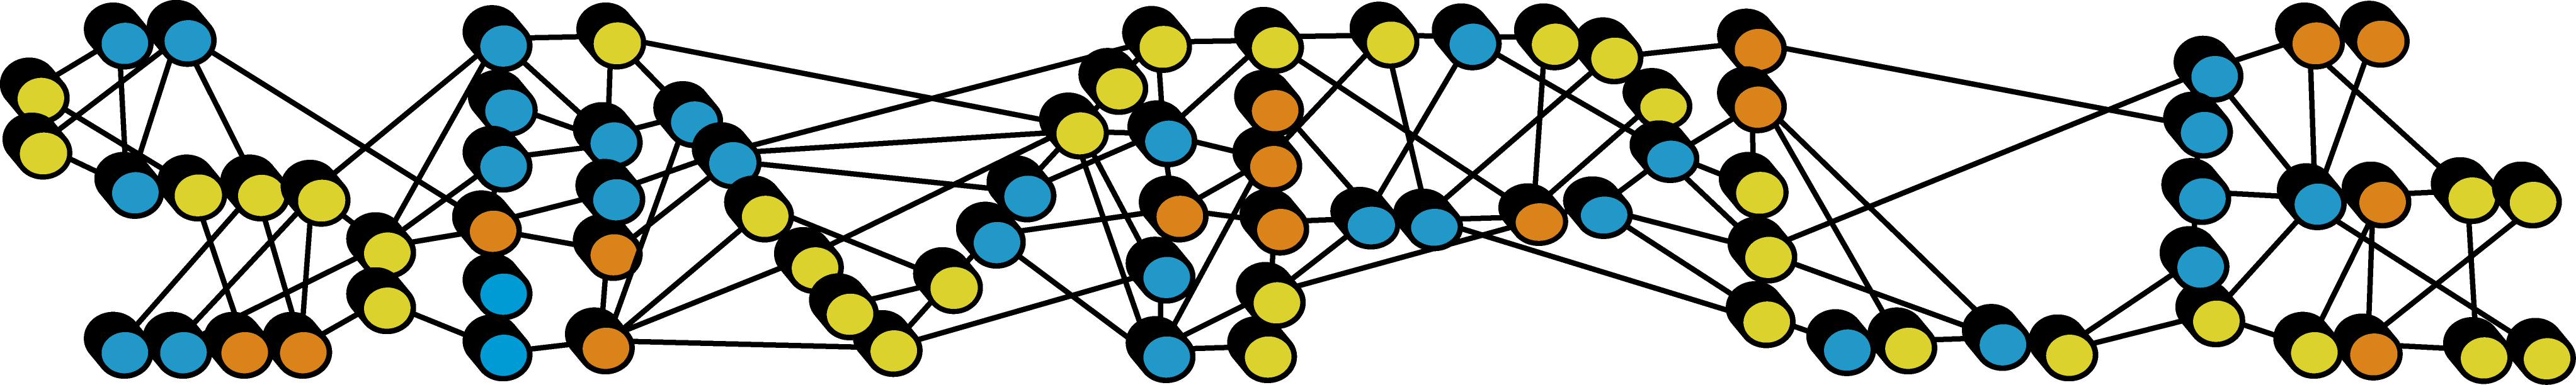
\includegraphics[keepaspectratio=true,scale=0.6]{./SIMPLE_logo/rawlogo}
%\caption{}
\end{figure}

\title{\prgname{Developers Guide to SIMPLE}}
\date{Christmas Day, 2016}
\author{Hans Elmlund}
\maketitle

\vspace{1em}
\begin{minipage}[ht]{0.48\textwidth}
\textbf{Contributors:}\\
cyril.reboul@monash.edu\\
dominika.elmlund@monash.edu\\
hans.elmlund@monash.edu\\
\textbf{Adress:}\\
Dept. Biochemistry and Molecular Biology\\
School of Biomedical Sciences\\
Monash University, Bldg. 77\\
Clayton, VIC, Australia, 3800\\
\textbf{Webpage:}\\
www.simplecryoem.com\\
\end{minipage}
\vspace{20pt}

\begin{quote}
\textbf{``Keep it SIMPLE stupid''}\\(\textit{Kelly Johnson}; lead engineer at the Lockheed Skunk Works, coined the famous KISS principle stating that systems work best if they are kept simple rather than made complex. Therefore, simplicity should be a key goal in design and unnecessary complexity should be avoided.)
\end{quote}

\begin{quote}
\textbf{``Everything should be made as SIMPLE as possible, but no SIMPLEr''}\\(\textit{Albert Einstein})
\end{quote}

\begin{quote}
\textbf{``Complex theories do not work, SIMPLE algorithms do''}\\(\textit{Vladimir N. Vapnik}; author of \textit{The Nature of Statistical Learning Theory})
\end{quote}
\clearpage

\tableofcontents{}
\clearpage

\section{Disclaimer}
Many of the general ideas/concepts presented in this document are not my original contributions but direct or modified rip-offs from other people's work, including Eric Evans' ``Domain-Driven Design, Tackling Complexity in the heart of Software'', the gang of four's classic work ``Design Patterns: Elements of Reusable Object-Oriented Software'', Damian Rouson's ``Scientific Software Design: The Object-oriented Way'' in addition to a number of Fortran language reference books. This document is therefore not intended for distribution but will serve as a guide for those developing code (or improving the model behind the code) within the SIMPLE environment.

\section{A Domain Model for SIMPLE Development}

\subsection{The Two Most Important Design Principles}
Before we start the esoteric discussion about object-oriented design philosophy, let's keep it simple. There are two principles of software design that have been repeated so many times in development documents and programming books that their origins are long forgotten. These are the two most important design principles, whether you are working on a fancy object-oriented library, hacking in procedural C code, writing a jiffy perl script or writing assembly code for a driver.
\begin{enumerate}
\item \textbf{DRY:} \textbf{D}on't \textbf{R}epeat \textbf{Y}ourself. No matter how convenient it is to cut and paste snippets of code and introduce some slight modifications when your head is buzzing with ideas and you want to test something NOW there is NEVER any justification for duplicating code. Repetitions are costly, they force you to update the same logics in multiple places in the library and it makes debugging a living hell. \textbf{DRY!!!}
\item \textbf{YAGNI:} \textbf{Y}ou \textbf{A}in't \textbf{G}onna \textbf{N}eed \textbf{I}t. A lot of time has been wasted in the name of completeness. Even if your clever maths routine can be tuned into accepting arrays of any shape or type, if the need that you have RIGHT NOW is for it to operate on real one-dimensional arrays, then only code the routine for the real one-dimensional arrays. Because chances are, if you extend it to all conceivable cases: \textbf{Y}ou \textbf{A}in't \textbf{G}onna \textbf{N}eed \textbf{I}t! And you end up with a lot of dead code in the library that those that come in as new developers will have to plow through and try to understand, only to realise they just wasted their time. Dead code should preferably never be written but if sections are dying as development progresses, better move them to a legacy folder of some sort.
\end{enumerate}

\subsection{One Team, One Language}
It is the nature of software to change, and SIMPLE has continued to evolve in the hands of the team that owns it. This document arouse as a consequence of the need for guiding design principles to keep the team focused and productive. SIMPLE is written in modern Fortran. It is crucial that every SIMPLE developer masters object-oriented Fortran 2008 programming. The core functionality of SIMPLE is accomplished by a set of layered classes that meet in modules that define their functional relationships and data sharing interconnections. Although these modules represent high-level abstractions that drive a lot of the functionality of the library, there are additional layers that serve to allow the simultaneous design of high-level workflows (user-oriented) and focused functionalities (expert-oriented) required for proper testing and effective development. Before we dig into the details of it all, I will describe the overall development and design philosophy of SIMPLE. The principles and guidelines outlined here are not necessarily implemented in the current version of SIMPLE but with common efforts and ruthless refactoring I believe that we will get there.

The phrase \textit{One Team, One Language} comes from Eric Evans' book on domain-driven design and has nothing to do with the programming language used. Instead, \textbf{it refers to the concept of \textit{ubiquitous language}. With a \textit{ubiquitous language}, conversations among developers, discussions among domain experts, and expressions in the code itself are all based on the same language, derived from a shared domain model.} Our domain model represents the steps required to process electron microscopy images of particles (biological as well as inorganic nanoparticles). The model should support analysis of particles of any symmetry (helical or point-group), accept images from any kind of microscope (200kV, 300kV, with or without phase-plate etc.) or electron detector, and be applicable to 2D (single-particle) and 3D (subtomographic averaging) particles alike. Currently, the support for tomography is weak (limited to motion-correction and dose-weighting of tomographic tilt-series) and substantial additional coding and refactoring of existing library parts will be required to support analysis of subtomograms with already established correlation/search/CTF methods. The model should furthermore support efficient parallel execution of SIMPLE on heterogeneous clusters and workstations, including hybrid CPU/GPU architectures, in a user-friendly manner.

\subsection{Modelling the Domain: Why Bother?}
If the coders don't feel responsible for the model, or don't understand how to make the theory underpinning the model work for an application, the model has nothing to do with the software. If developers don't realise that changing the code changes the model, then their refactoring will weaken the model rather than strengthening it. Meanwhile, when a modeler is separated from the implementation process, he or she never acquires or quickly loses, a feel for the constraints of the implementation. \textbf{The basic constraint of \textit{model-driven design} is that the model supports an effective implementation and abstracts key domain knowledge. The knowledge and skills of experienced designers will  be transferred to other developers if the division of labour allows the kind of collaboration that conveys the subtleties of coding a \textit{model-driven design}.} Currently, the two most experienced model-driven SIMPLE coders are Cyril and Hans. The reason for this is that we have invested 50/50 into the model (I want to solve an accurate \textit{ab initio} structure with EM) and the code that expresses the model. When additional collaborators/coders enter the team, it is important that we explain the principles even though we cannot expect that everyone will invest equally into the model and the code. For example, Dominika is 100\% model at the moment but I do anticipate that Alex will start contributing to the code base and the scientific programmer that we will employ will have to focus a large part of his/her initial efforts into understanding the model. Anyone responsible for changing code must learn to express the model through the code. Every developer must be involved in some level of discussion about the model and have regular contact with domain experts (many of which are our users). Those who contribute in different ways must consciously engage those who touch the code in a dynamic exchange of model ideas through the \textit{ubiquitous language}.

\subsection{The Layered SIMPLE Architecture}
Partition a complex program into layers. Develop a design within each layer that is cohesive and that depends only on the layers below. Follow standard architectural patterns to provide loose coupling to the layers above. Concentrate all the code related to the domain model in one layer and isolate it from the user interface, application and infrastructure code. The domain objects, free of the responsibility of displaying themselves, storing themselves, managing application tasks, and so forth, can be focused on expressing the domain model. This allows a model to evolve to be rich enough and clear enough to capture essential research knowledge and put it into work. SIMPLE was designed in a layered fashion.
\newpage{}
\begin{SCfigure}[][h]
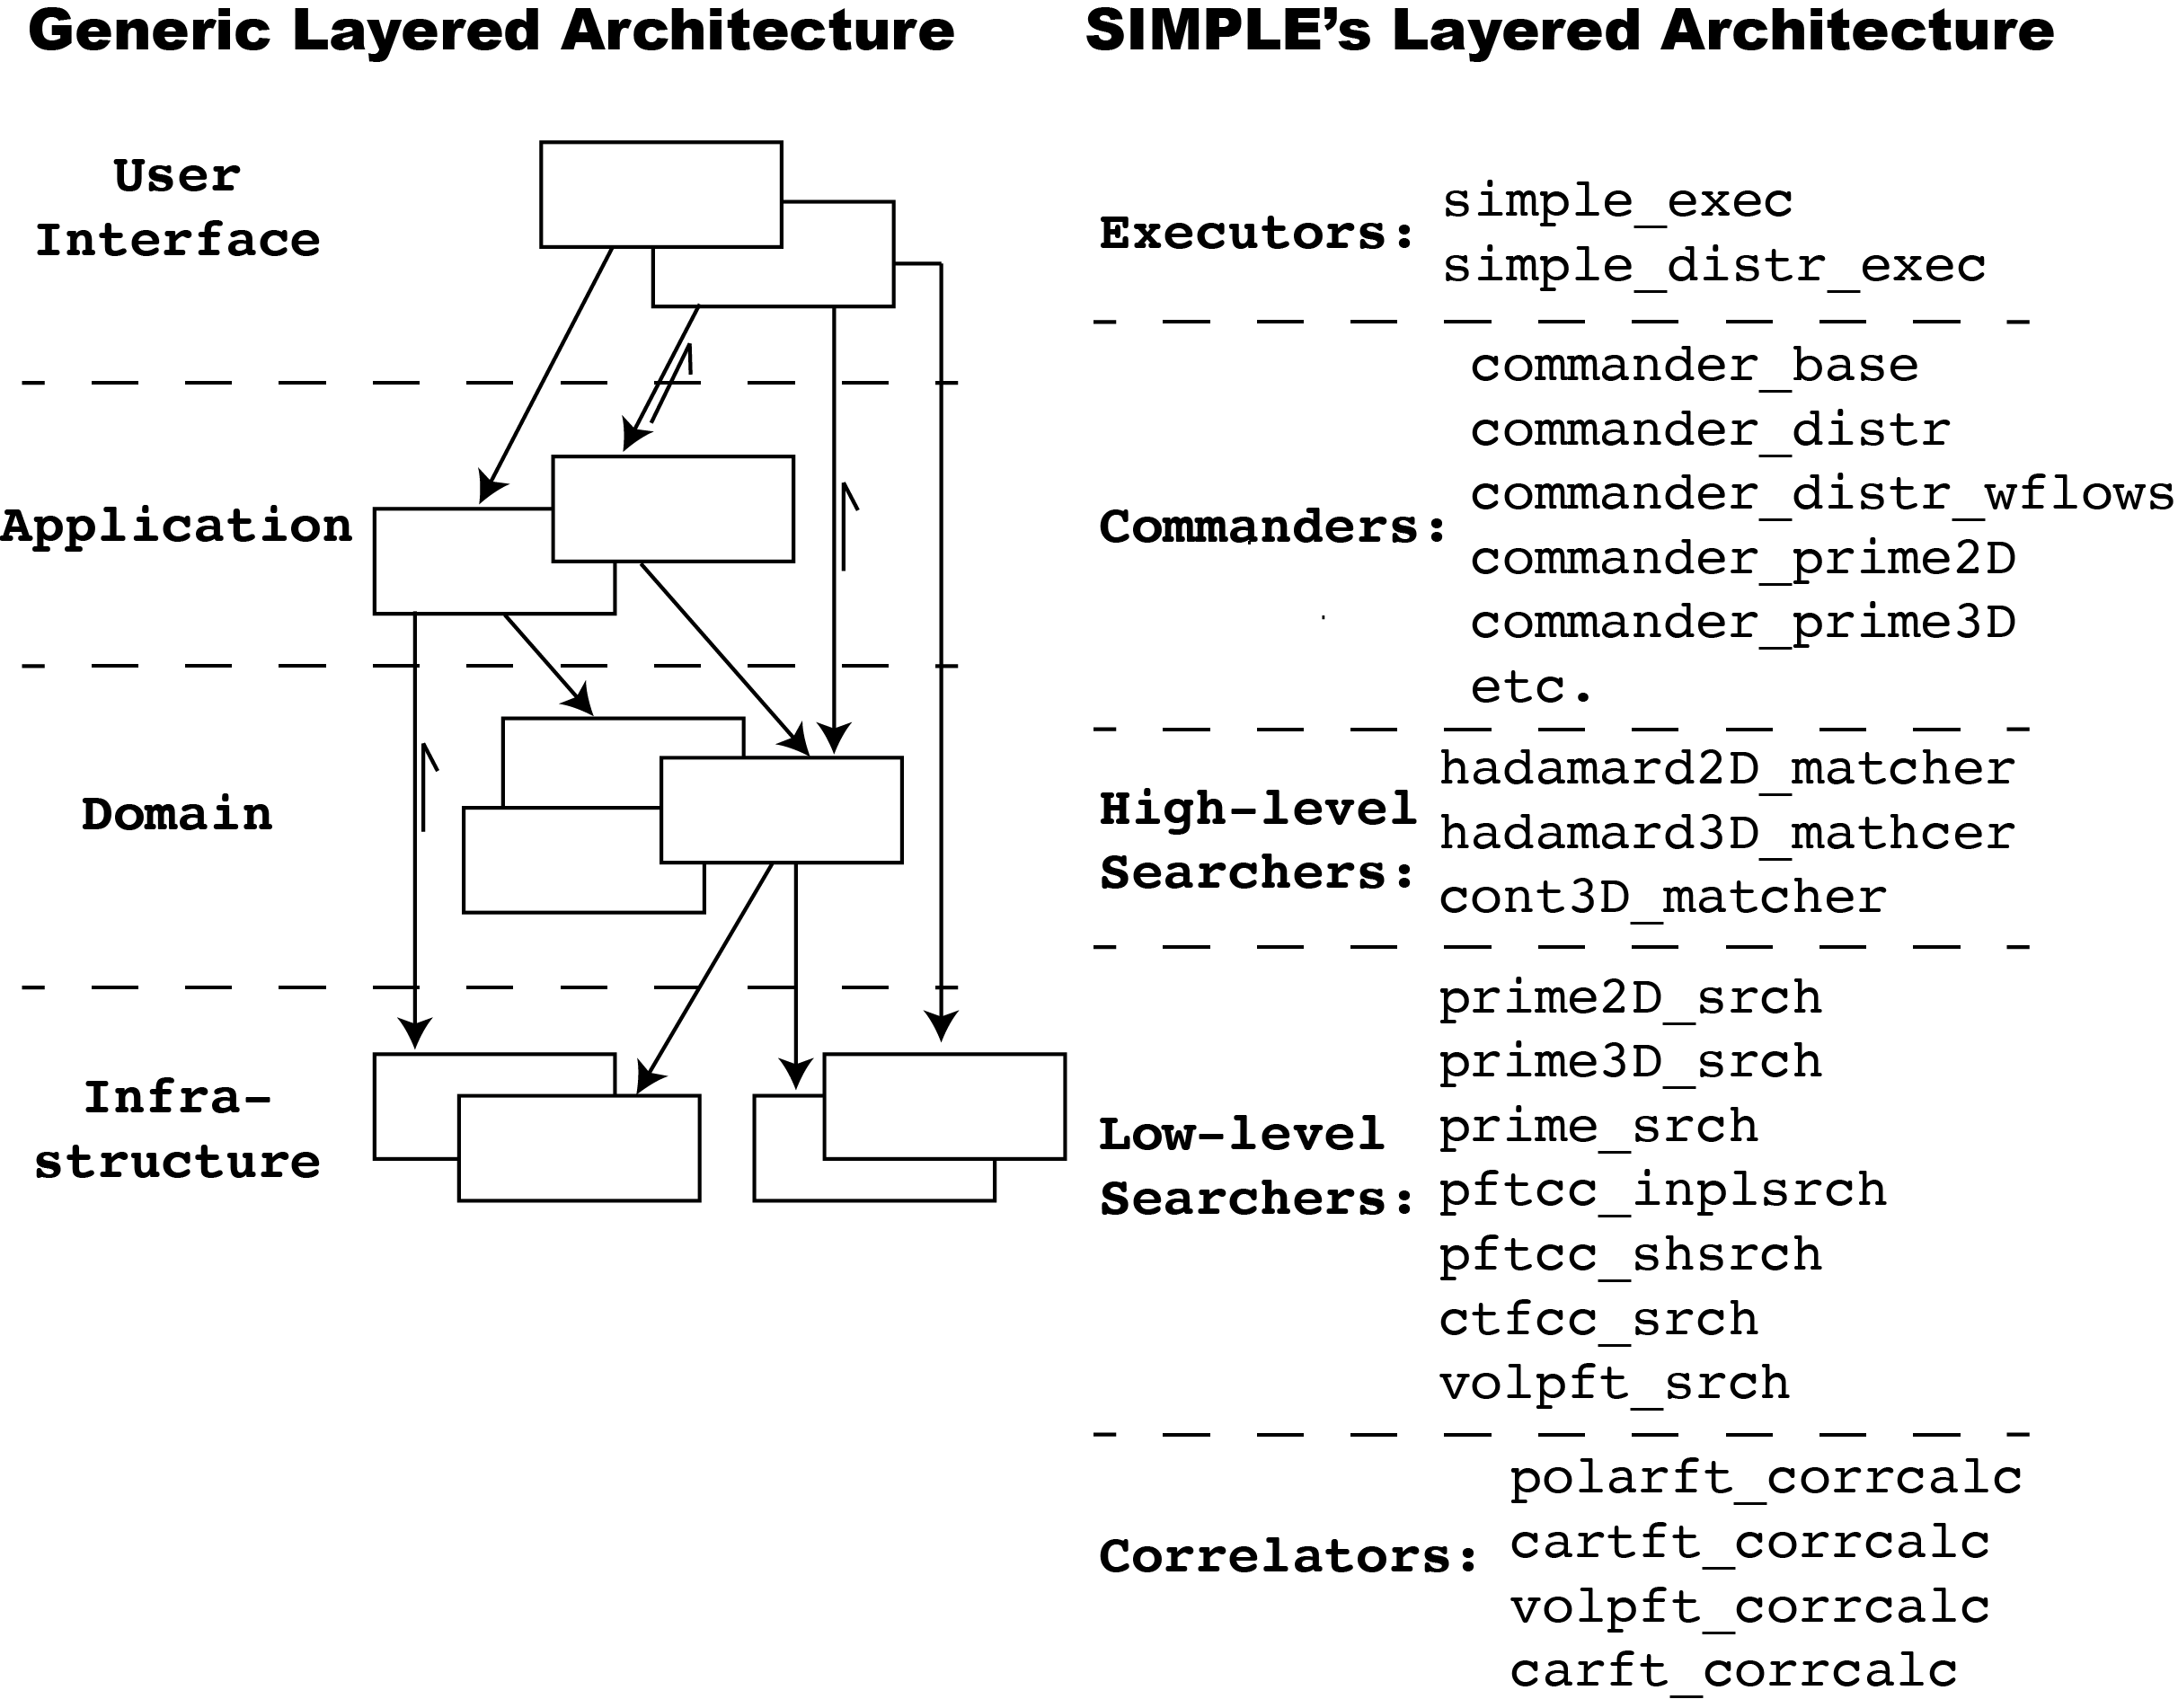
\includegraphics[keepaspectratio=true,scale=0.6]{./LayeredArch/layered_arch}
\end{SCfigure}

Layering the design was not something that we really thought long and hard about. The layered structure evolved as a natural consequence of creating units that express fundamental components of the domain model. At the root level are the correlators that evaluate the goal function (correlation) in different settings.
\begin{verbatim}
simple_cartft_corrcalc.f90   ! calculates correlations between 2D Cartesian FTs
simple_comlin_corr.f90       ! calculates common line correlations
simple_polarft_corrcalc.f90  ! calculates correlations between 2D polar FTs 
simple_volpft_corrcalc.f90   ! calculates correlation between volume FTs
\end{verbatim}
These classes have very few dependencies, the most notable one being the builder. These are the number crunchers of the SIMPLE library. About 60\% of the computations in the the PRIME2D/3D searches consists of calculating correlations. It is in this area we will focus our efforts in performance enhancement by designing data structures that make efficient use of cache and data structures that scale up the matrix sizes so that the calculations can be efficiently done on GPUs. In the next level up are the low-level searchers.
\begin{verbatim}
simple_cftcc_srch.f90     ! continuous search using cartesian FTs
simple_comlin_srch.f90    ! basic common lines search routines
simple_comlin_symsrch.f90 ! symmetry search routines
simple_ft_shsrch.f90      ! origin shift search for Cartesian FTs
simple_ftexp_shsrch.f90   ! fast origin shift search using expanded Cartesian FTs
simple_pftcc_inplsrch.f90 ! discrete/continuous in-plane parameter polar FT search
simple_pftcc_shsrch.f90   ! origin shift search for polar FTs
simple_prime2D_srch.f90   ! search routines used in PRIME2D
simple_prime3D_srch.f90   ! search routines used in PRIME3D
simple_prime_srch.f90     ! search routines common to PRIME2D/3D
simple_symsrcher.f90      ! symmetry axis search routines
simple_volpft_srch.f90    ! volume registration search routines
\end{verbatim}
The most prominent role of these classes is to put together the correlators with the classes responsible for the optimisation. The most important and highest level aggregate classes in this group are the \texttt{prime2D\_srch} and \texttt{prime3D\_srch} classes who shares common functionality via the \texttt{prime\_srch} class. In order to understand the algorithmic details of the stochastic optimisation implemented in the PRIME algorithm, look in the \texttt{prime2D\_srch} and \texttt{prime3D\_srch} classes. In the next level we find the classes executing the projection-matching-based algorithms.
\begin{verbatim}
simple_cont3D_matcher.f90      ! continuous projection matching
simple_hadamard2D_matcher.f90  ! discrete 2D clustering and alignment
simple_hadamard3D_matcher.f90  ! discrete 3D ab initio reconstruction
\end{verbatim}
Most designs would now have ended with a final layer of executables with an associated user interface. However, in SIMPLE we use a trick based on a design pattern called \textit{commander} (described below) to ``objectify'' the execution of a program. This means that the abstract concept of ``executing PRIME2D'' is encapsulated in a class that can be instantiated to create objects. The commander classes have only a single method ``execute''. Why bother complicating things in this manner? Because now we can create arrays of executables and we can systematically vary the input parameters and make a computer program that automatically does this for us. This, of course, has fundamental implications for the design of unit tests or restart methodologies. It also makes it possible to create high level workflows that combine virtually every functionality of the library. Moreover, it lends itself readily to highly efficient job scheduling in cluster environments and on workstations. By studying the commander classes in SIMPLE we get a feel for the high-level functionalities and how they can be combined to create advanced and highly automated workflows.
\begin{verbatim}
simple_commander_base.f90          ! the abstract base class
simple_commander_checks.f90        ! simple check commanders
simple_commander_comlin.f90        ! common lines commanders
simple_commander_distr.f90         ! commanders used in distributed execution
simple_commander_distr_wflows.f90  ! the parallel high-level workflows
simple_commander_imgproc.f90       ! basic image processing commanders
simple_commander_mask.f90          ! masking commanders
simple_commander_misc.f90          ! miscellaneous commanders
simple_commander_oris.f90          ! orientation commanders
simple_commander_preproc.f90       ! pre-processing commanders
simple_commander_prime2D.f90       ! prime2D commanders
simple_commander_prime3D.f90       ! prime3D commanders
simple_commander_rec.f90           ! volume reconstruction commanders
simple_commander_sim.f90           ! simulation commanders
simple_commander_volops.f90        ! miscellaneous volume operation commanders
\end{verbatim}
Lastly, we have the executable layer.
\begin{verbatim}
simple_exec       ! shared-memory parallelisation mode
simple_distr_exec ! hybrid distributed/shared-memory parallelisation mode 
\end{verbatim}
The distinction between these two execution routes will be explained in detail below.

\section{The Building Blocks of SIMPLE}

\subsection{SIMPLE Classes}
<input>

\subsection{SIMPLE Design Patterns}
In every area of design\textemdash{}houses, cars, rowboats, or software\textemdash{}we build on patterns that have been found to work in the past, improvising within established themes. Sometimes we have to invent something completely new. But by basing standard elements on patterns, we avoid wasting our energy on problems with known solutions so that we can focus on our unusual needs. Also, building from conventional patterns helps us avoid creating a design so idiosyncratic that it is difficult to talk about it.

<check Ruby book for descriptions>
<aggregate>

Aggregates tighten up the model itself by defining clear ownership and boundaries, avoiding a chaotic, tangled web of objects. This pattern is crucial to maintaining integrity in all phases of the life cycle of a domain object. 

<builder>
<factory>
<commander>
<decorator>
<singleton>
 
\subsection{SIMPLE Modules}
Modules are an old, established design element that plays a key role in modern Fortran. The Fortran module is technically implementing a singleton design pattern, \textit{i.e.} there can be only one instance of a module, it does not need to be instantiated and the data declared in the header of the module (not in the subroutines and functions) exist throughout the execution of the program. Everyone uses modules but few treat them as a full-fledged part of the model. Code gets broken down into all sorts of categories, from aspects of the technical architecture to developers' work assignments. Even developers who refactor a lot tend to content themselves with modules conceived early in the project.

It is a truism that there should be low coupling between modules and high cohesion within them. Explanations of coupling and cohesion tend to make them sound like technical metrics, to be judged mechanically based on the distributions of associations and interactions. Yet it isn't just code being divided into modules, but concepts. There is a limit to how many things a person can think about at once (hence low coupling). Incoherent fragments of ideas are as hard to understand as an undifferentiated soup of ideas (hence high cohesion). Well-chosen modules bring together elements of the model with particularly rich conceptual relationships. This high cohesion of objects with related responsibilities allows modelling and design work to concentrate within a single module, a scale of complexity a human mind can easily handle. When you place some classes together in a module, you are telling the next developer who looks at your design to think about them together, as a team working together toward a common goal. If your model is telling a story (about how to process single-particle images), the modules are chapters.

\textbf{Choose modules that tell a story about the system and contain a cohesive set of concepts. This often yield low coupling between modules, but if it doesn't, look for a way to change the model to disentangle the concepts, or search for an overlooked concept that might be the basis of a module that would bring elements together in a meaningful way. Seek low coupling in the sense of concepts that can be understood and reasoned about independently of each other. Refine the model until it partitions according to high-level domain concepts and the corresponding code is decoupled as well.}

Give modules names that become part of the \textit{ubiquitous language}. Modules and their names should reflect insight into the domain.

\section{Refactoring Toward Deeper Insight}

\subsection{Making Implicit Concepts Explicit}
A deep, well-constructed model has power because it contains the central concepts and abstractions that can succinctly and flexibly express essential knowledge of the user's activities, their problems, and their solutions. The first step is to somehow represent the essential concepts of the domain in the model. Refinement comes later, after successive iterations of knowledge crunching and refactoring. But this process really gets into gear when an important concept is recognised and made explicit in the model and design.

\textbf{Many transformations of domain models and the corresponding code happen when developers recognise a concept that has been hinted at in discussion or present implicitly in the design, and they then represent it explicitly in the model with one or more objects or relationships.}

Listen to the language the domain experts (the electron microscopists) use. Are there terms that succinctly state something complicated? Are they correcting your word choice (perhaps diplomatically)? Do the puzzled looks on their faces go away when you use a particular phrase? These are hints of a concept that will for sure benefit the model. When the users or domain experts use vocabulary that is nowhere in the design, that's a warning sign. It is a doubly strong warning when both the developers and the domain experts are using terms that are not in the design.

\subsection{Supple Design}
Supple is an adjective that means ``bending and moving easily and gracefully; flexible''. The ultimate purpose of software is to serve users. But first, that same software has to serve developers. This is especially true in a process that emphasises refactoring. I assume here that the reader knows that refactoring entails much more than simply renaming functions and subroutines. Refactoring is the process of moving bits and pieces of code around, making it logically consistent, readable and with naming consistent with the domain model. This should be done without changing the program's external behaviour. Succesful refactoring strongly depends on having well-designed automatic unit tests (discussed below). Ruthless refactoring is a key component of the extreme programming paradigm and it is best done in paris, with one coder overlooking the shoulder of the other.

\textbf{When software doesn't have a clean design, developers dread even looking at the existing mess or making a change that could aggravate the tangle or break something through an unforeseen dependency. To have a project accelerate as development proceeds\textemdash{}rather than get weighted down by its own legacy\textemdash{}demands a design that is a pleasure to work with, inviting to change. A supple design.}

A lot of overengineering has been justified in the name of flexibility. But more often than not, excessive layers of abstraction and indirection get in the way. Look at the design of software that really empowers the people who handle it; you will usually see something simple. Simple is not easy. To create elements that can be assembled into elaborate systems and still be understandable, a dedication to \textit{model-driven design} has to be joined with a moderately rigorous design style.

\begin{SCfigure}[][h]
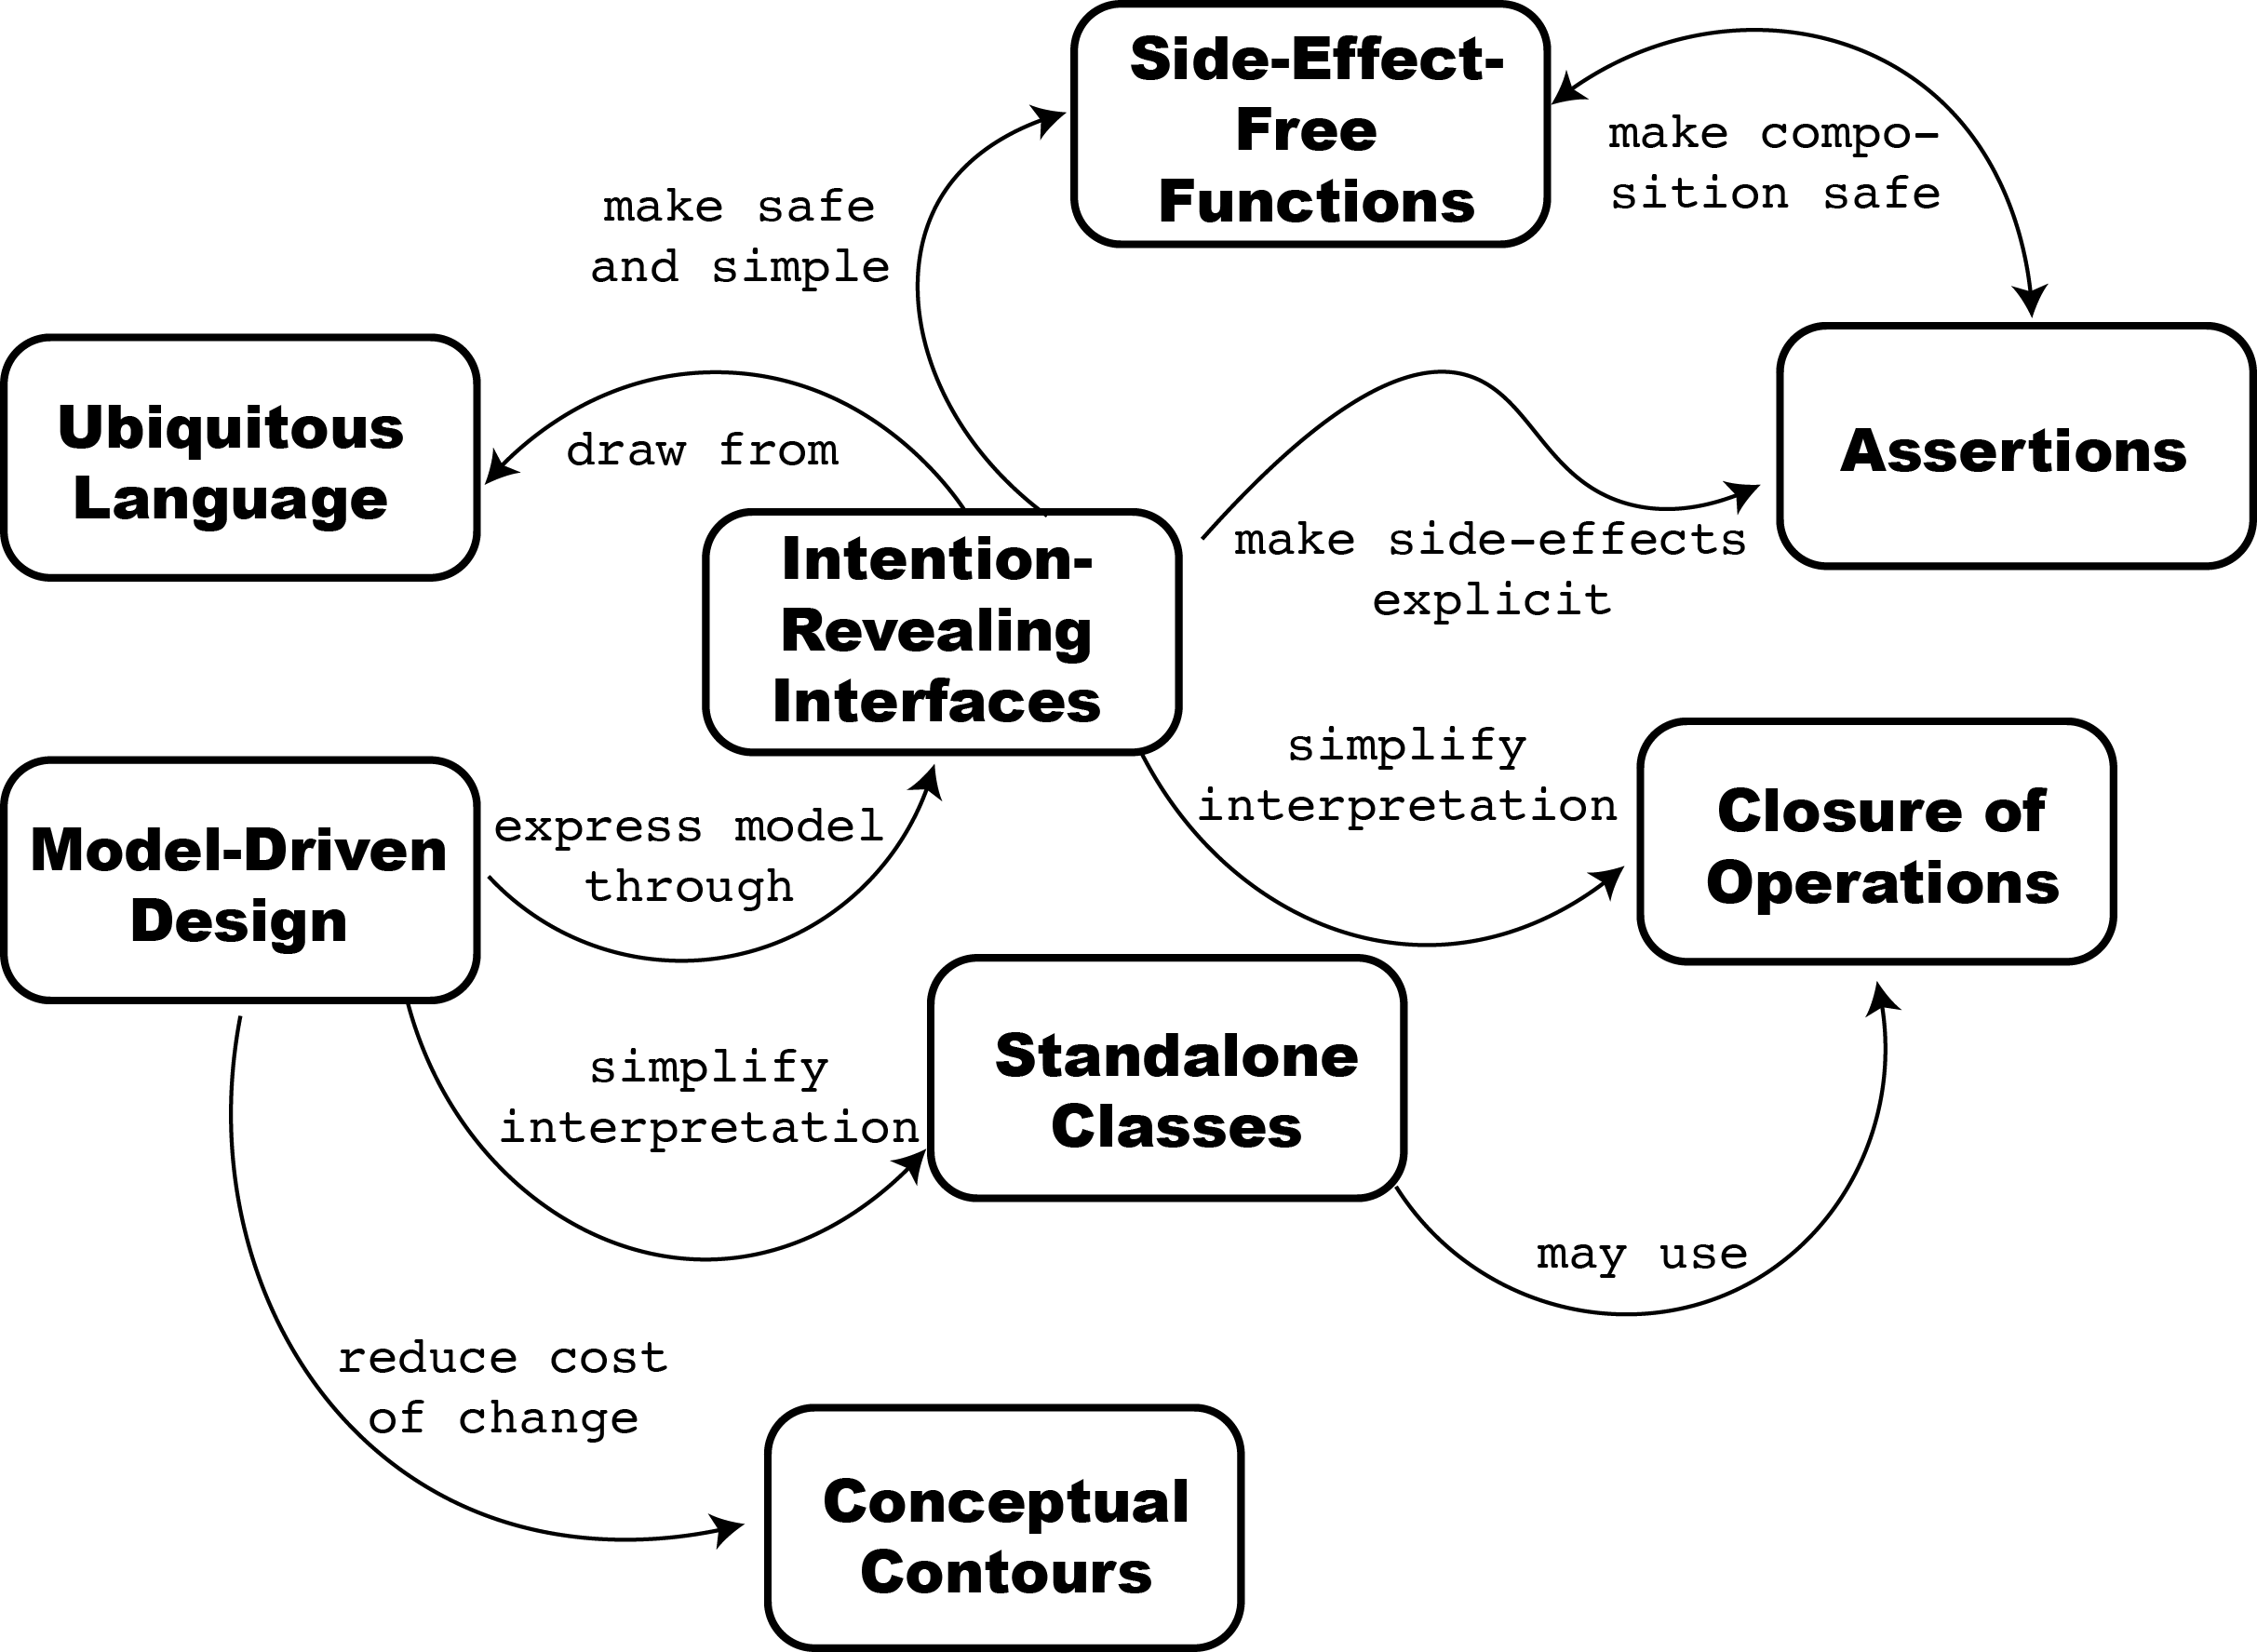
\includegraphics[keepaspectratio=true,scale=0.6]{./SuppleDesign/SuppleDesign}
\caption{Some patterns that contribute to supple design.}
\end{SCfigure}

\subsection{Intention-Revealing Interfaces}
If a developer must consider the implementation of a component in order to use it, the value of encapsulation is lost. If someone other than the original developer must infer the purpose of an object or operation based on its implementation, that new developer may infer a purpose that the operation or class fulfils only by chance. If that was not the intent, the code may work for a moment, but the conceptual basis of the design will have been corrupted, and the two developers will be working at cross-purpose.

Name classes and operations to describe their effect and purpose, without reference to the means by which they do what they promise. This relieves the client of the need to understand the internals. These names should conform to the \textit{ubiquitous language} so that team members can quickly infer their meaning. I tend to try to keep names short, not because my limited memory prevents me to use long method names, but because the code becomes a mess to read when names are too long.

\subsection{Side-Effect-Free Functions}
Place as much of the logic of a program into functions, operations that return results with no observable side-effects. This can be enforced by the use of pure and elemental functions in modern Fortran (example below)

\begin{verbatim}
!>  \brief  this metric is measuring the frobenius deviation from the identity
!!          matrix .in.[0,2*sqrt(2)] Larochelle, P.M., Murray, A.P., Angeles, J., 
!!          A distance metric for finite sets of rigid-body displacement in the 
!!          polar decomposition. ASME J. Mech. Des. 129, 883?886 (2007)
pure real function geodesic_dist( self1, self2 )
    class(ori), intent(in) :: self1, self2
    real :: Imat(3,3), sumsq, diffmat(3,3)
    Imat      = 0.
    Imat(1,1) = 1.
    Imat(2,2) = 1.
    Imat(3,3) = 1.
    diffmat = Imat-matmul(self1%rmat,transpose(self2%rmat))
    sumsq   = sum(diffmat*diffmat)
    if( sumsq > 0.0001 )then
        geodesic_dist = sqrt(sumsq)
    else
        geodesic_dist = 0.
    endif
end function geodesic_dist
\end{verbatim}


Strictly segregate commands (methods that result in modifications to observable state) into very simple operations that do not return domain information. Further control side effects by moving complex logic into \textit{value objects} when a concept fitting the responsibility presents itself.

\subsection{Assertions}
In contrast to for example Java or C++, Fortran isn't really equipped with any good tools to deal with assertions and Fortran programmers generally feel uneasy when plowing through code scattered with assert statements. In SIMPLE, we have never coded assertions directly into our classes. Instead, we rely on a set of automated unit tests (described below) which admittedly needs to be extended to test more code than it currently does. 

\subsection{Conceptual Contours}
Sometimes developers chop functionality fine to allow flexible combination. Sometimes they lump it large to encapsulate complexity. Sometimes they seek a consistent granularity, making all classes and operations to a similar scale. These are oversimplifications that don't work well as a general rule. As a rule of thumb, if you method call has more than three arguments (excluding the object instance), chances are you are lumping it too large. On the other hand, when performance is important and the embedded algorithm will be subjected to parallelisation, substantial performance gains may follow from merging operations and reduce overheads due to thread creation, data transfer to devices etc. However, remember the famous quote by Donald Knuth ``Premature optimisation is the root of all evil''. Therefore:

\textbf{Decompose design elements (operations, interfaces, classes and aggregates) into cohesive units, taking into consideration your intuition of the important divisions in the domain. Observe the axes of change and stability through successive refactorings and look for the underlying \textit{conceptual contours} that explain these shearing patterns. Align the model with the consistent aspects of the domain that make it a viable area of knowledge in the first place.}

The goal is a simple set of interfaces that combine logically to make sensible statements in the \textit{ubiquitous language}, and without the distraction and maintenance burden of irrelevant options. This is typically an outcome of refactoring: it's hard to produce up front. But it may never emerge from technically oriented refactoring; it emerges from refactoring toward deeper insight. The \texttt{simple\_ctf} class is an example of a successfully encapsulated functionality. It also represents a standalone class (discussed below).

\begin{verbatim}
module simple_ctf
use simple_defs ! singleton
implicit none

public :: ctf, test_ctf
private

type ctf
    private
    real    :: smpd        = 0.    !< sampling distance (A)
    real    :: kV          = 0.    !< acceleration voltage (kV) 
    real    :: Cs          = 0.    !< spherical aberration (mm)
    real    :: wl          = 0.    !< wavelength (A)
    real    :: amp_contr   = 0.07  !< fraction of amplitude contrast ([0.07,0.15])
    real    :: dfx         = 0.    !< underfocus x-axis (microns)
    real    :: dfy         = 0.    !< underfocus y-axis (microns)
    real    :: angast      = 0.    !< azimuth of x-axis 0.0 means (degrees)
    real    :: phaseq      = 0.    !< phase contrast weight (derived constant)
    real    :: ampliq      = 0.    !< amplitude contrast weight (derived constant)
  contains
    ! INITIALISER
    procedure, private :: init
    ! CTF EVALUATION
    procedure          :: eval
    procedure, private :: evalPhSh
    procedure, private :: eval_df
    ! CTF APPLICATION
    procedure          :: ctf2img
    procedure          :: ctf2spec
    procedure          :: apply
    ! CALCULATORS
    procedure          :: freqOfAZero
    procedure, private :: solve4PhSh
    procedure, private :: sqFreq4PhSh
    procedure, private :: sqSf4PhSh
end type

interface ctf
    module procedure constructor
end interface
\end{verbatim}

\subsection{Standalone Classes}
\textbf{Even within a module, the difficulty of interpreting a design increases wildly as dependencies are added. This adds to mental overload, limiting the design complexity a developer can handle. Implicit concepts contribute to this load even more than explicit references.}

Refined models are distilled until every remaining connection between concepts represents something fundamental to the meaning of those concepts. In an important subset, the number of dependencies can be reduced to zero, resulting in a class that can be understood all by itself, along with a few primitives and basic library concepts.

\textbf{Low coupling is fundamental to object design. When you can, go all the way. Eliminate \textit{all} other concepts from the picture. Then the class will be completely self-contained and can be studied and understood alone. Every such self-contained class significantly eases the burden of understanding a module.}

Dependencies on other classes within the same module is less harmful than those outside. Likewise, when two objects are naturally tightly coupled, multiple operations involving the same pair can actually clarify the relationship. The goal is not to eliminate all dependencies, but to eliminate all nonessential ones.

\section{Maintaining Model Integrity}
Although we seldom think about it explicitly, the most fundamental requirement of a model is that it be internally consistent; that its terms always have the same meaning, and that it contain no contradictory rules. The internal consistency of a model, such that each term is unambiguous and no rules contradict, is called \textit{unification}. A model is meaningless unless it is logically consistent. In an ideal world, we would have a single model spanning the whole domain of the research field. This model would be unified, without any contradictory or overlapping definitions of terms. Every logical statement about the domain would be consistent. 

\subsection{Continuous Integration}
It is very hard to maintain the level of communication needed to develop a unified system of any size. We need ways of increasing communication and reducing complexity. We also need safety nets that prevent overcautious behaviour, such as developers duplicating functionality because they are afraid that they will break existing code. Of equal importance to prevent such undesired behaviours is that all developers are reaching a certain level of understanding of the system. Naturally, certain developers will have areas where they excel but there is a knowledge threshold that all the developers in the team must pass. We also need to respect the rules of the framework and in the same time not being afraid of introducing changes. It is a delicate balance. The team must cultivate a shared understanding of the ever-changing model. Practices may help, but the most fundamental one is to constantly update the \textit{ubiquitous language} definition. SIMPLE developers use Git for step-by-step, reproducible merge/build and automated test suites (both described below). Development sometimes occurs in spurts and sometimes stagnates, depending on the current workload of the team. However, we must strive to merge all code frequently and relentlessly exercise the  \textit{ubiquitous language} to hammer out a shared view of the model as the concepts evolve in different people's heads.

\section{The SIMPLE Compilation Environment}

\section{The SIMPLE Test Environment}

\section{Creating A SIMPLE Application}

\section{Debugging in SIMPLE}

\section{Distributing SIMPLE on Workstations and Clusters}

\section{The SIMPLE Git Repository}

\section{Concluding Remarks}

\end{document}